\newpage
\hypertarget{initialize vis}{}
\subsection{Establishing the visual TGG}
\visHeader

\begin{itemize}

\item[$\blacktriangleright$] Given that TGGs can only successfully execute if the involved metamodels are in the same working set, double-click your
\texttt{Dict\-ion\-ary.eap} file to open it in Enterprise Architect (EA). The unexpanded project broswer should resemble Fig.~\ref{ea:mocaTagged}.
As you can see, the project is already populated with the source \texttt{MocaTree} specification for a generic tree structure.

\begin{figure}[htpb]
\begin{center}
  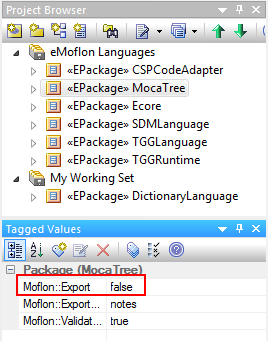
\includegraphics[width=0.4\textwidth]{ea_mocaTaggedValues}
  \caption{figureCaption}
  \label{ea:mocaTagged}
\end{center}
\end{figure}

\end{itemize}

If you inspect the tagged values\footnote{The ``Tagged Values'' window can be opened by going to ``View/Tagged Values''} for each language, you'll notice that
the \texttt{MocaTree} package has the \texttt{Moflon::Export} value set to \texttt{false}. This ensures that the package is \emph{ignored} when exporting. As
with all standard metamodels (e.g., Ecore or the SDM metamodel) the \texttt{MocaTree} package in EA should be regarded as read-only, required only in the
EA project so that SDMs can refer to the classes defined in the package. The corresponding Java code is provided by our Eclipse plugin and added automatically
to the Java build path whenever necessary.

\begin{itemize}

\item[$\blacktriangleright$] Go ahead and inspect the \texttt{MocaTree} metamodel diagram (Fig.~\ref{ea:mocaTree}). It basically combines concepts from a
filesystem (folders and files), XML concepts (text-only nodes and attributes), and a general indexed\footnote{The index attribute in \texttt{TreeElement} can be used to
demand a certain \emph{order} of nodes in an SDM, which is otherwise not guaranteed by default (in general, order is non-deterministic).} containment
hierarchy.

\begin{figure}[htpb]
\begin{center}
  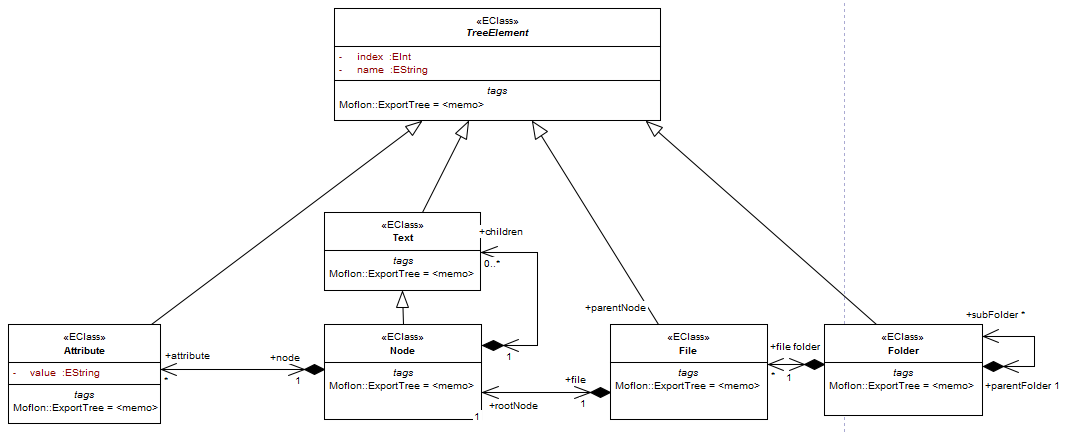
\includegraphics[width=\textwidth]{ea_metamodelMocaTree}
  \caption{The MocaTree Metamodel}
  \label{ea:mocaTree}
\end{center}
\end{figure}

\item[$\blacktriangleright$] Let's begin our TGG. Add a new package to the \texttt{My Working Set} node named \texttt{Dict\-ion\-ary\-Code\-Adap\-ter}. Add a
new TGG schema diagram (Fig\texttt{ea:newTGGDiagram}) with the same name.

\begin{figure}[htpb]
\begin{center}
  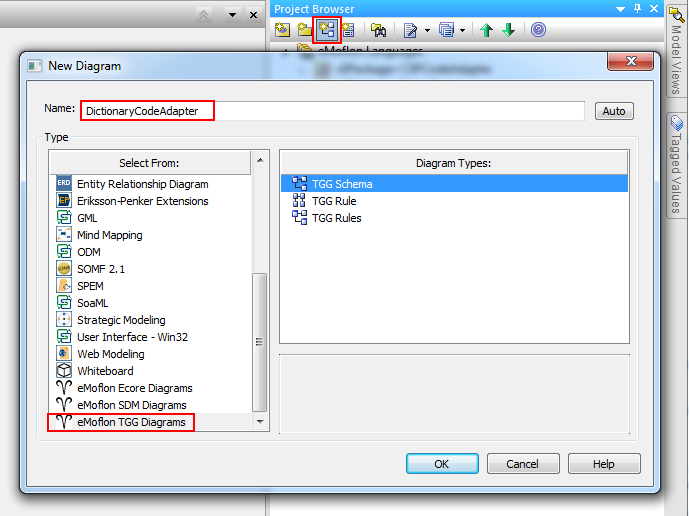
\includegraphics[width=0.85\textwidth]{ea_adapterTGGDiagram}
  \caption{Create a new TGG Diagram}
  \label{ea:newTGGDiagram}
\end{center}
\end{figure}

\end{itemize}

Our conventions and workflow state that this \emph{code adapter} is a package that contains the tree-to-model transformation logic. This could be integrated
directly in the corresponding metamodel (\texttt{Dic\-tion\-ary\-Language}), but here a separation makes sense as there could be \emph{different} code adapters
for the \emph{same} language.

\begin{itemize}

\item[$\blacktriangleright$] In the next dialogue, set the source project as \texttt{MocaTree} and the target project as \texttt{Dict\-ion\-ary\-Lang\-uage}.

\item[$\blacktriangleright$] As a final step to ensure the package exports correctly to the Eclipse workspace as a TGG, add a single correspondence type between
\texttt{Folder} and \texttt{Library} by performing a drag-and-drop gesture of the elements into your schema diagram.\footnote{To review how to do this, refer to
Part IV, Section \update.} Your diagram should now resemble Fig.~\ref{ea:firstCorrType}.

\vspace{0.5cm}

\begin{figure}[htpb]
\begin{center}
  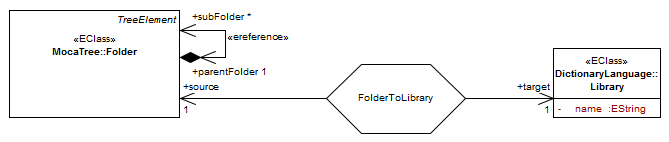
\includegraphics[width=\textwidth]{ea_firstAdapterCorrespondence}
  \caption{The transformation's first correspondence type}
  \label{ea:firstCorrType}
\end{center}
\end{figure}

\item[$\blacktriangleright$] Save and validate your file via the eMoflon control panel.\footnote{Introducted in Part \update, Section \update.} Switch back
to Eclipse and refresh the package exlporer. A new \texttt{Dict\-ion\-ary\-Code\-Adap\-ter} folder should have been generated for the TGG EPackage. Your
workspace is nearly complete!

\jumpSingle{subSec:setupParser}

\end{itemize}
